% Auto-generated by the analysis pipeline — do not edit
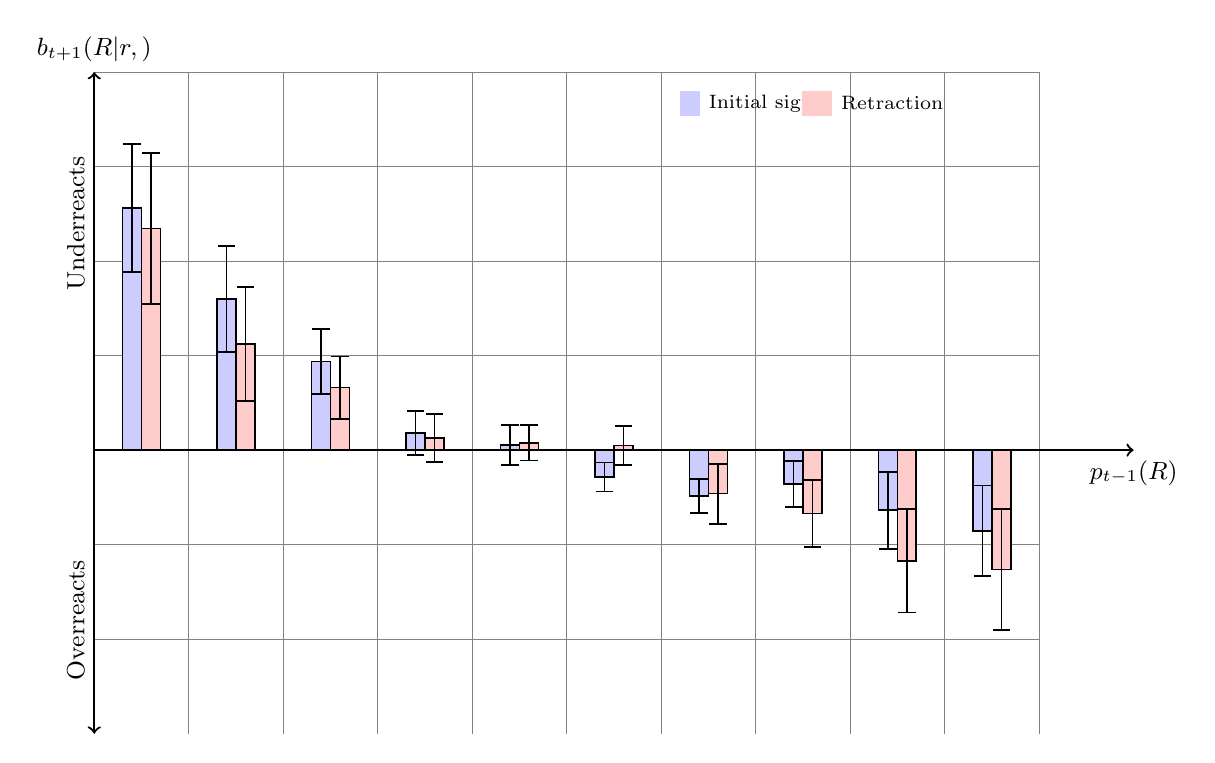
\begin{tikzpicture}[scale=12]
\draw[help lines,step=0.1] (0,-0.3) grid (1,0.4);
\filldraw[opaque,white!80!blue] (0.0300,0) rectangle (0.0500,0.2560);
\draw[line width=0.6] (0.0300,0) rectangle (0.0500,0.2560);
\draw[line width=0.6,|-|] (0.0400,0.1873) -- (0.0400,0.3247);
\filldraw[opaque,white!80!red] (0.0500,0) rectangle (0.0700,0.2345);
\draw[line width=0.6] (0.0500,0) rectangle (0.0700,0.2345);
\draw[line width=0.6,|-|] (0.0600,0.1537) -- (0.0600,0.3152);
\filldraw[opaque,white!80!blue] (0.1300,0) rectangle (0.1500,0.1599);
\draw[line width=0.6] (0.1300,0) rectangle (0.1500,0.1599);
\draw[line width=0.6,|-|] (0.1400,0.1028) -- (0.1400,0.2170);
\filldraw[opaque,white!80!red] (0.1500,0) rectangle (0.1700,0.1122);
\draw[line width=0.6] (0.1500,0) rectangle (0.1700,0.1122);
\draw[line width=0.6,|-|] (0.1600,0.0511) -- (0.1600,0.1732);
\filldraw[opaque,white!80!blue] (0.2300,0) rectangle (0.2500,0.0937);
\draw[line width=0.6] (0.2300,0) rectangle (0.2500,0.0937);
\draw[line width=0.6,|-|] (0.2400,0.0587) -- (0.2400,0.1287);
\filldraw[opaque,white!80!red] (0.2500,0) rectangle (0.2700,0.0661);
\draw[line width=0.6] (0.2500,0) rectangle (0.2700,0.0661);
\draw[line width=0.6,|-|] (0.2600,0.0320) -- (0.2600,0.1001);
\filldraw[opaque,white!80!blue] (0.3300,0) rectangle (0.3500,0.0180);
\draw[line width=0.6] (0.3300,0) rectangle (0.3500,0.0180);
\draw[line width=0.6,|-|] (0.3400,-0.0061) -- (0.3400,0.0421);
\filldraw[opaque,white!80!red] (0.3500,0) rectangle (0.3700,0.0126);
\draw[line width=0.6] (0.3500,0) rectangle (0.3700,0.0126);
\draw[line width=0.6,|-|] (0.3600,-0.0136) -- (0.3600,0.0388);
\filldraw[opaque,white!80!blue] (0.4300,0) rectangle (0.4500,0.0054);
\draw[line width=0.6] (0.4300,0) rectangle (0.4500,0.0054);
\draw[line width=0.6,|-|] (0.4400,-0.0170) -- (0.4400,0.0277);
\filldraw[opaque,white!80!red] (0.4500,0) rectangle (0.4700,0.0077);
\draw[line width=0.6] (0.4500,0) rectangle (0.4700,0.0077);
\draw[line width=0.6,|-|] (0.4600,-0.0120) -- (0.4600,0.0274);
\filldraw[opaque,white!80!blue] (0.5300,0) rectangle (0.5500,-0.0286);
\draw[line width=0.6] (0.5300,0) rectangle (0.5500,-0.0286);
\draw[line width=0.6,|-|] (0.5400,-0.0448) -- (0.5400,-0.0124);
\filldraw[opaque,white!80!red] (0.5500,0) rectangle (0.5700,0.0048);
\draw[line width=0.6] (0.5500,0) rectangle (0.5700,0.0048);
\draw[line width=0.6,|-|] (0.5600,-0.0166) -- (0.5600,0.0261);
\filldraw[opaque,white!80!blue] (0.6300,0) rectangle (0.6500,-0.0487);
\draw[line width=0.6] (0.6300,0) rectangle (0.6500,-0.0487);
\draw[line width=0.6,|-|] (0.6400,-0.0674) -- (0.6400,-0.0300);
\filldraw[opaque,white!80!red] (0.6500,0) rectangle (0.6700,-0.0461);
\draw[line width=0.6] (0.6500,0) rectangle (0.6700,-0.0461);
\draw[line width=0.6,|-|] (0.6600,-0.0788) -- (0.6600,-0.0135);
\filldraw[opaque,white!80!blue] (0.7300,0) rectangle (0.7500,-0.0357);
\draw[line width=0.6] (0.7300,0) rectangle (0.7500,-0.0357);
\draw[line width=0.6,|-|] (0.7400,-0.0609) -- (0.7400,-0.0105);
\filldraw[opaque,white!80!red] (0.7500,0) rectangle (0.7700,-0.0672);
\draw[line width=0.6] (0.7500,0) rectangle (0.7700,-0.0672);
\draw[line width=0.6,|-|] (0.7600,-0.1035) -- (0.7600,-0.0310);
\filldraw[opaque,white!80!blue] (0.8300,0) rectangle (0.8500,-0.0637);
\draw[line width=0.6] (0.8300,0) rectangle (0.8500,-0.0637);
\draw[line width=0.6,|-|] (0.8400,-0.1053) -- (0.8400,-0.0222);
\filldraw[opaque,white!80!red] (0.8500,0) rectangle (0.8700,-0.1171);
\draw[line width=0.6] (0.8500,0) rectangle (0.8700,-0.1171);
\draw[line width=0.6,|-|] (0.8600,-0.1726) -- (0.8600,-0.0616);
\filldraw[opaque,white!80!blue] (0.9300,0) rectangle (0.9500,-0.0853);
\draw[line width=0.6] (0.9300,0) rectangle (0.9500,-0.0853);
\draw[line width=0.6,|-|] (0.9400,-0.1340) -- (0.9400,-0.0365);
\filldraw[opaque,white!80!red] (0.9500,0) rectangle (0.9700,-0.1265);
\draw[line width=0.6] (0.9500,0) rectangle (0.9700,-0.1265);
\draw[line width=0.6,|-|] (0.9600,-0.1913) -- (0.9600,-0.0617);
\draw[line width=0.8,->]  (0,0) -- (1.1,0) node[below] {\small{$p_{t-1}(R)$}};
\draw[line width=0.8,<->] (0,-0.3) -- (0,0.4) node[above] {\small{$b_{t+1}(R|r,\xmark)$}};
\draw (0,0.24) node[above,rotate=90] {\small{Underreacts}};
\draw (0,-0.18) node[above,rotate=90] {\small{Overreacts}};
\filldraw[white!80!blue] (0.62,0.3540) rectangle (0.64,0.3790);
\node[right] at (0.64,0.3670) {\scriptsize{Initial signal}};
\filldraw[white!80!red] (0.75,0.3540) rectangle (0.78,0.3790);
\node[right] at (0.78,0.3670) {\scriptsize{Retraction}};
\end{tikzpicture}
